
%(BEGIN_QUESTION)
% Copyright 2012, Tony R. Kuphaldt, released under the Creative Commons Attribution License (v 1.0)
% This means you may do almost anything with this work of mine, so long as you give me proper credit

Skisser den grafiske tolkningen av den deriverte $dy \over dx$ i punktet som er angitt i grafen (den røde prikken), og avgjør om verdien er {\it positiv} eller {\it negativ}:

$$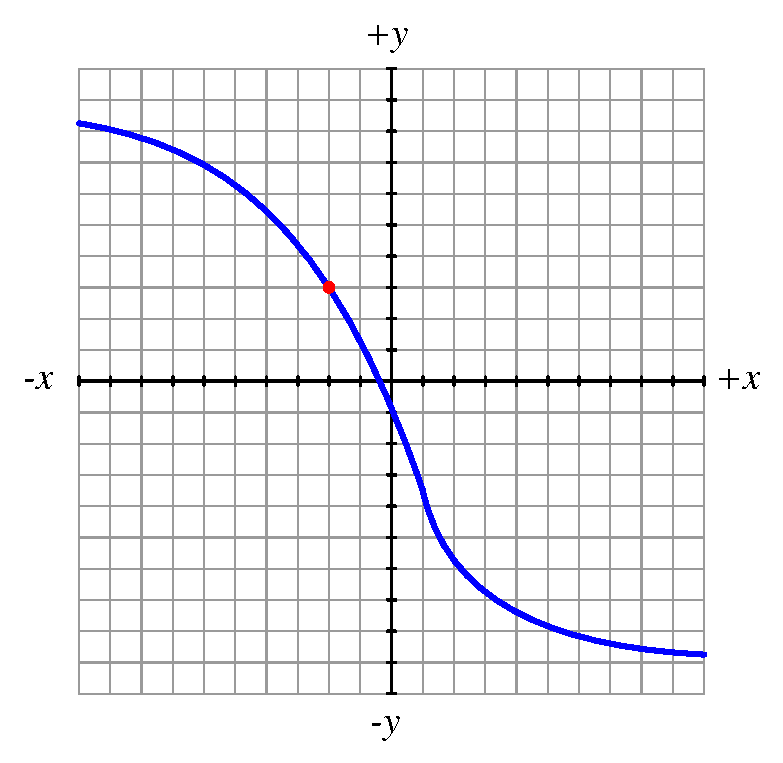
\includegraphics[width=15.5cm]{i01347x01.eps}$$

\underbar{file i01347}
%(END_QUESTION)





%(BEGIN_ANSWER)

$$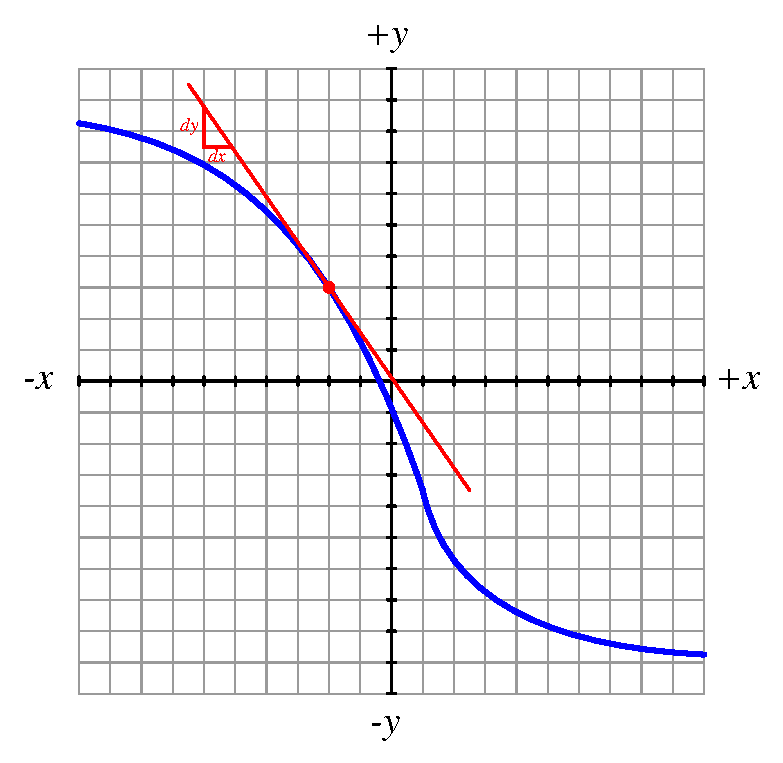
\includegraphics[width=15.5cm]{i01347x02.eps}$$

$dy \over dx$ har en {\it negativ} verdi ved den røde prikken, fordi differensialet $dy$ er negativt mens differensialet $dx$ er positivt.

%(END_ANSWER)





%(BEGIN_NOTES)


%INDEX% Mathematics, calculus: derivative (defined in a graphical sense)

%(END_NOTES)

